\newpage \section{The TEPX upgrade for HL-LHC}
\label{sec:tepx}
(describe the TEPX detector design, algorithms clusters/coincidences, D4R1 as HL-LHC luminometer, stat precision, linearity)\\

The High Luminosity (HL)-LHC will increase instantaneous luminosity to unprecedented value of $7.5 \times 10^{34} cm^{-2} s^{-1}$ which corresponds to 200 proton-proton collisions per bunch crossing (pileup). Run 2 pixel detector will not be able to handle the extreme radiation environment, resolve nearby particle tracks and operate properly to give a reliable estimate of the instantaneous luminosity for high pileup values. That is why it will be replaced by a new pixel detector which will be composed of three subdetectors: tracker barrel pixel detector (TBPX), tracker forward pixel detector (TFPX) and tracker endcap pixel detector (TEPX). TEPX will have better radiation tolerance, increased granularity, improved two-track separation, improved estimation of hit rate and statistical precision, extended tracking acceptance $|\eta|=4$ with Disk 4 Ring 1 operating as an independent luminometer. \\

Tracker endcap pixel detector (TEPX) consists of four double disks per side (-Z and +Z) as shown in Fig. 27 with each double disk containing five rings as shown in Fig. 28 having 20, 28, 36, 44 and 48 modules respectively. One double disk has four surfaces with +Z side containing modules with even module number in front layers (L1 $\&$ L2) and modules with odd module number in back layers (L3 $\&$ L4) from Ring 1 to Ring 4 and for Ring 5, modules with odd module number in front layers and modules with even module number in back layers as shown in Fig. 29. For -Z side, four surfaces contain modules with odd module number in front layer and modules with even module number in back layer from Ring 1 to Ring 4 and for Ring 5, modules with even module number in front layer and modules with odd module number in back layer. \\


Instantaneous luminosity determination using PCC method for Phase 2 HL-LHC can be based on counting the number of clusters or coincidences. The innermost ring of the last disk of TEPX (D4R1) is located at 2.65 m away from the interaction point that is beyond the tracking acceptance ($|\eta = 4|$) and as this region has few tracking points, it can be solely used for the purpose of luminosity measurement by using the full available trigger rate and bandwidth.  Two fold coincidences are those hits which are created by the module overlap regions between various layers of one TEPX double disk. Two fold coincidences are better way to distinguish between a real hit and random electrical noise. They are more likely to be real hit than random electrical noise. Two fold coincidence in $\phi$ will involve modules overlapping in the same ring in front and back layers of one double disk as shown in top part of Fig. 30 and Fig. 31 while two fold coincidence in r will require modules overlapping between successive rings in the front (L1 $\&$ L2) and back layers (L3 $\&$ L4) of one double disk as shown in bottom part of Fig. 30. Luminosity calculated based on counting coincidences has an advantage over clusters that afterglow effects are tiny in the case of coincidences. \\


Nonlinearity is one of the systematic uncertainty in the calculation of instantaneous luminosity using PCC and PCC visible cross section $\sigma_{vis}$. A linear relation between the number of clusters and pileup (PU) would imply that\\

$<N_{cluster/interaction}> = \frac{<N_{cluster}>}{(PU)} = \frac{\sigma_{visible}}{\sigma_{interaction} (\sqrt{s})}$ \\

$<N_{cluster}> =  \frac{\sigma_{visible}}{\sigma_{interaction}(\sqrt{s})} (PU)$ \\

\newpage Linearity indicates that the PCC visible cross section $\sigma_{vis}$ does not depend on the per bunch instantaneous luminosity (ideal luminometer). In ideal  scenario, $\sigma_{vis}$ is not dependent on pileup, but this a potential problem with the luminometer. A non-linear relation $<N_{cluster}> = \alpha (PU)^{\gamma}, \gamma \neq 1$ would add non-linear terms in the rate equation $R = \sigma L$  and cause $\sigma_{vis}$ to vary with the per bunch instantaneous luminosity and pileup values.


\begin{figure}[H]
  \centering
  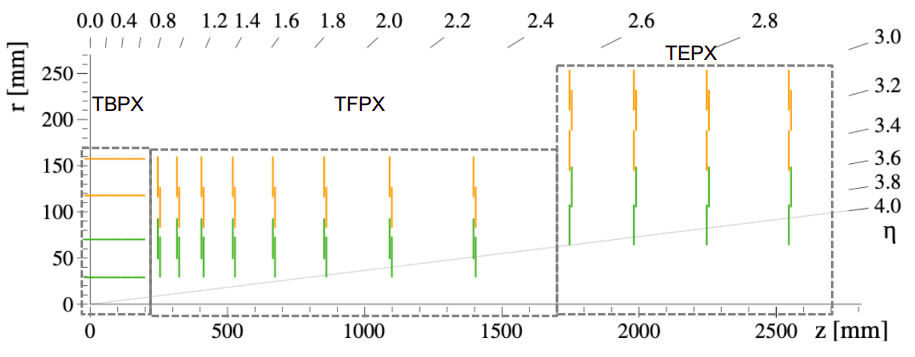
\includegraphics[width=0.8\columnwidth]{./tepx_geometry.png}
  \caption{ \onehalfspacing A layout of the CMS Phase-2 inner tracker showing four TEPX disks, eight TFPX disks and 4 barrel layers.}
  \label{fig:CMS}
\end{figure}


\begin{figure}[H]
  \centering
  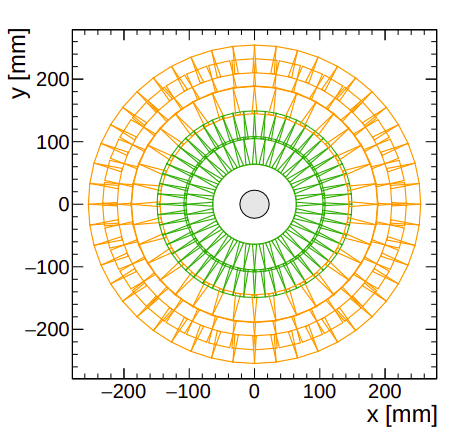
\includegraphics[width=0.5 \columnwidth]{./xydisc.png}
  \caption{ \onehalfspacing Sketch of the TEPX Disk layouts in x-y view. Modules of type 1 $\times$ 2 are shown in green, while 2 $\times$ 2 modules are represented in orange.}
  \label{fig:CMS}
\end{figure}

\begin{figure}[H]
  \centering
  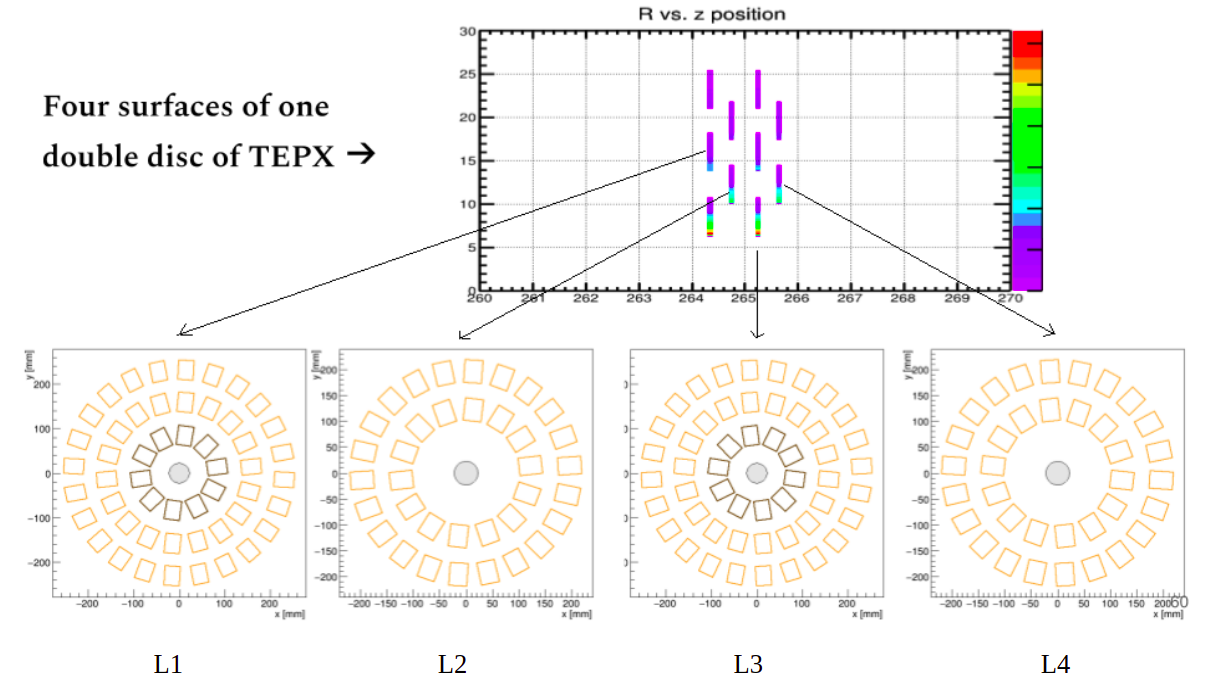
\includegraphics[width=1 \columnwidth]{./fourlayers.png}
  \caption{ \onehalfspacing Fours layers of one double disk of TEPX showing module arrangement in rings for all layers.}
  \label{fig:CMS}
\end{figure}




\begin{figure}[H]
  \centering
  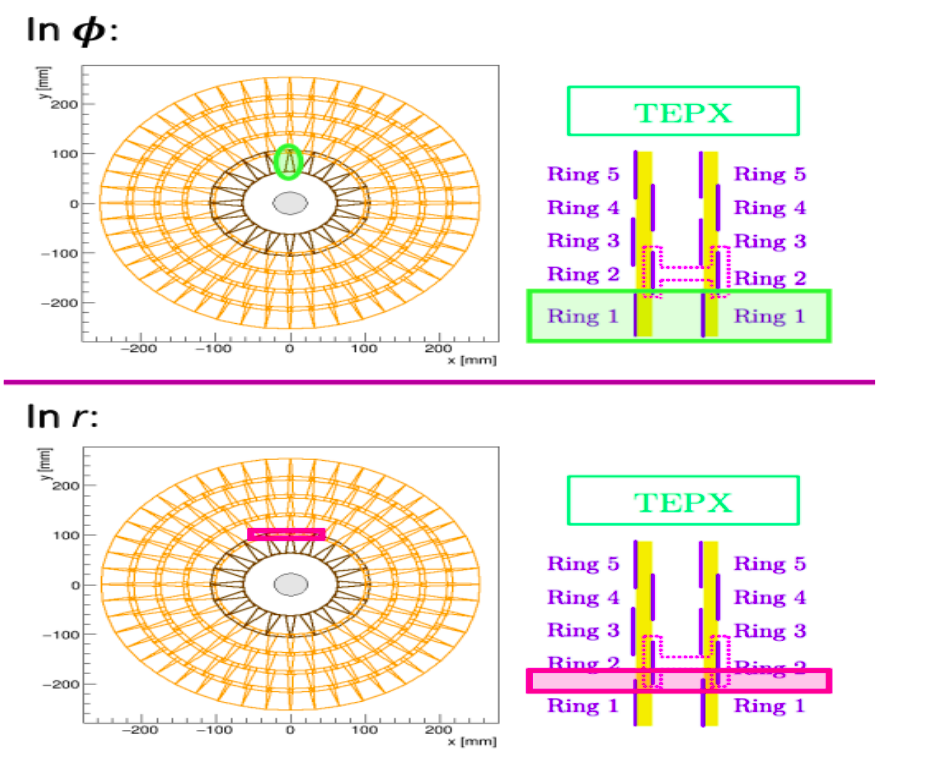
\includegraphics[width=0.8\columnwidth]{./coincidences.png}
  \caption{ \onehalfspacing Diagram showing modules overlap between the front and back layers of one double disk of TEPX that creates two fold coincidences in $\phi$ and r.}
  \label{fig:CMS}
\end{figure}

\begin{figure}[H]
  \centering
  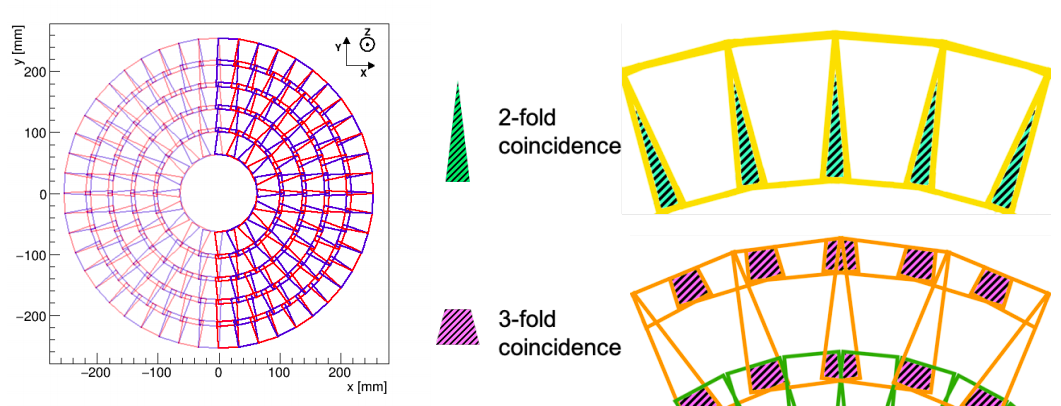
\includegraphics[width=0.8\columnwidth]{./up.png}
  \caption{\onehalfspacing Left: View in the x-y plane of the double disk structure of one TEPX disk. The sensors in blue and red correspond to the two double disks at slightly different z positions. Right: Example of two- and threefold coincidence regions on a portion of a single TEPX disk.}
  \label{fig:CMS}
\end{figure}


\newpage
\begin{figure}[H]
  \centering
  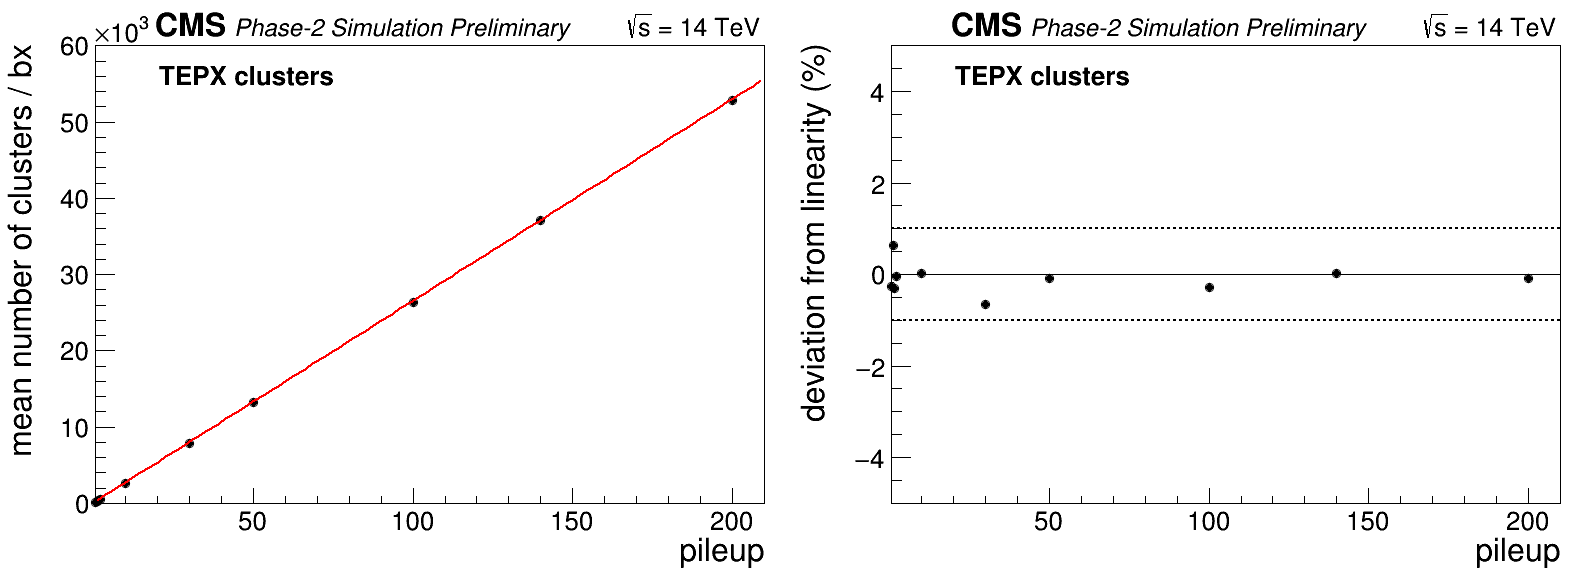
\includegraphics[width=1\columnwidth]{./totalclusters.png}
  \caption{\onehalfspacing Left: Simulated mean number of clusters for all entire TEPX detector as a function of pileup. A line is fitted between pileup values of 0 and 2, and then extrapolated up to a pileup of 200. Right: Deviation from linearity for clusters for entire TEPX detector. The non-linearity is calculated as the relative difference between the data points and the values of the fit function at the respective pileup value. Non-linearity is within 1 \% for entire pileup range. Pileup 200 corresponds to High Luminosity (HL)-LHC environment.}
  \label{fig:CMS}
\end{figure}



\begin{figure}[H]
  \centering
  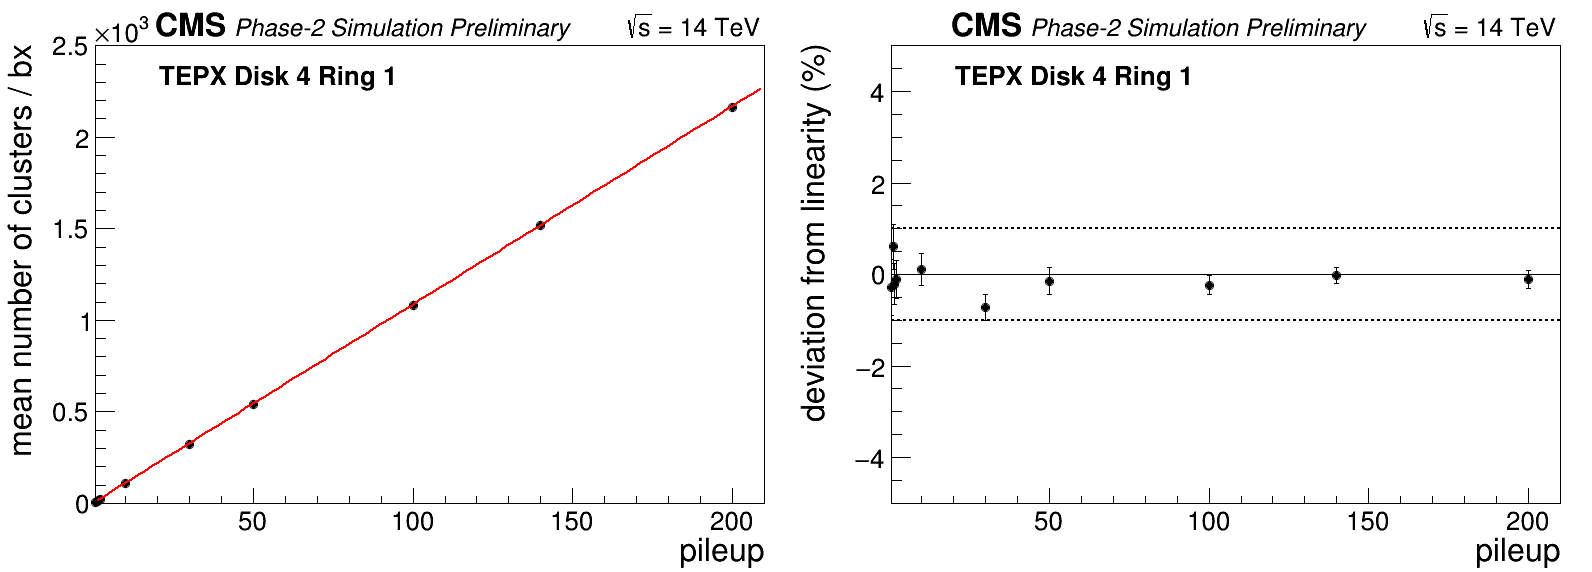
\includegraphics[width=1\columnwidth]{./clustersD4R1.png}
  \caption{\onehalfspacing Left: Simulated mean number of clusters for TEPX Disk 4 Ring 1 as a function of pileup. Right: Deviation from linearity for clusters for TEPX Disk 4 Ring 1. The non-linearity is calculated as the relative difference between the data points and the values of the fit function at the respective pileup value.}
  \label{fig:CMS}
\end{figure}



\begin{figure}[H]
  \centering
  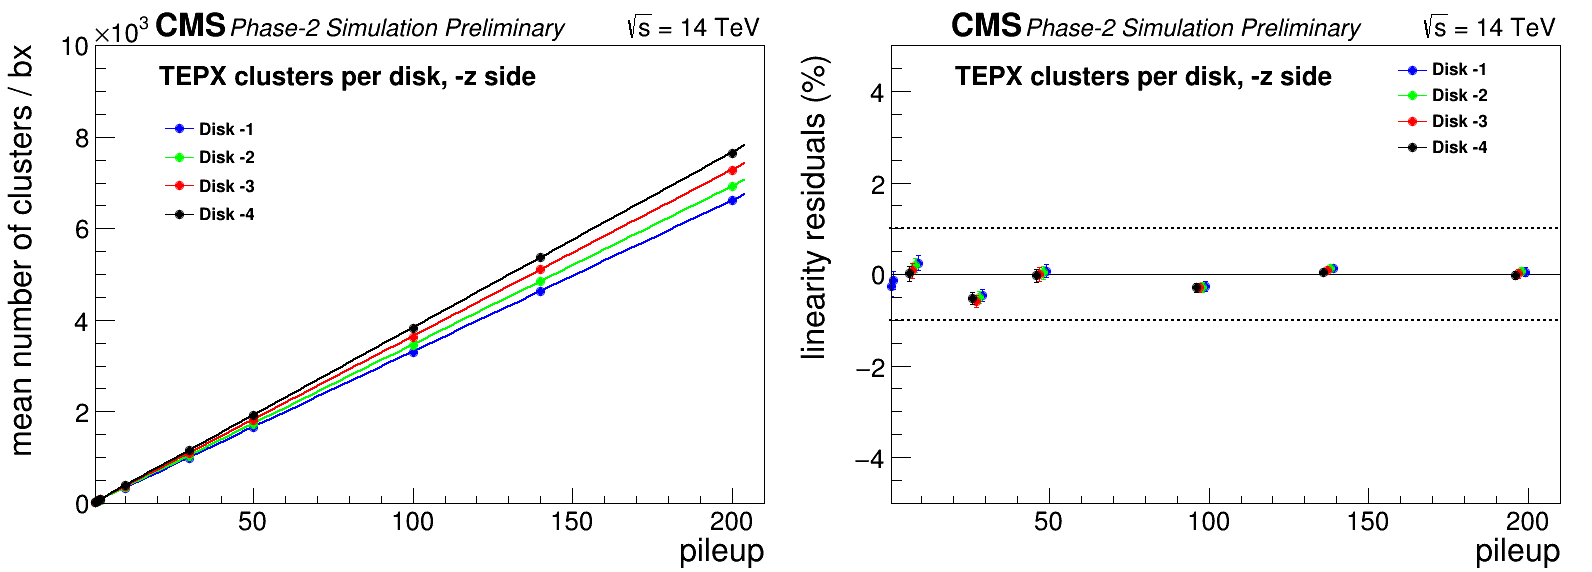
\includegraphics[width=1 \columnwidth]{./clustersperdisk-z.png}
  \caption{Left: Simulated mean number of clusters for -z side TEPX disks as a function of pileup. Right: Deviation from linearity for clusters for -z side TEPX disks.}
  \label{fig:CMS}
\end{figure}


\begin{figure}[H]
  \centering
  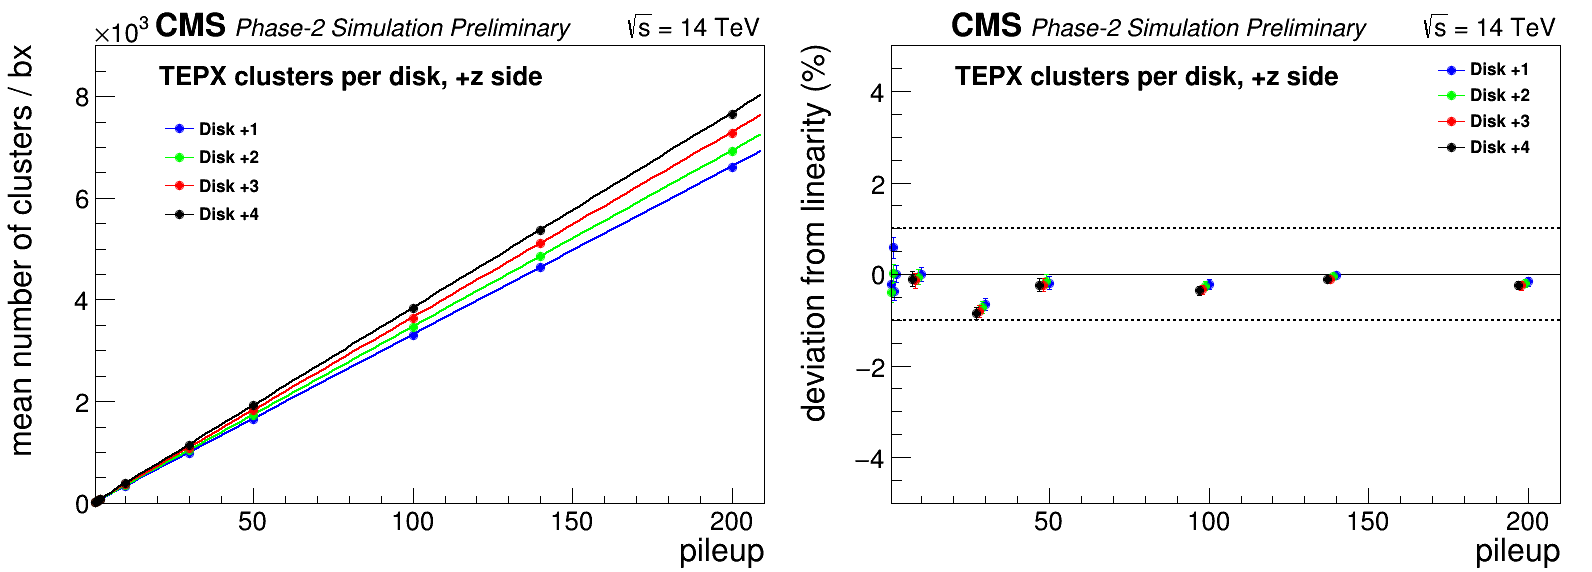
\includegraphics[width=1 \columnwidth]{./clustersperdisk+z.png}
  \caption{Left: Simulated mean number of clusters for +z side TEPX disks as a function of pileup. Right: Deviation from linearity for clusters for +z side TEPX disks.}
  \label{fig:CMS}
\end{figure}


\begin{figure}[H]
  \centering
  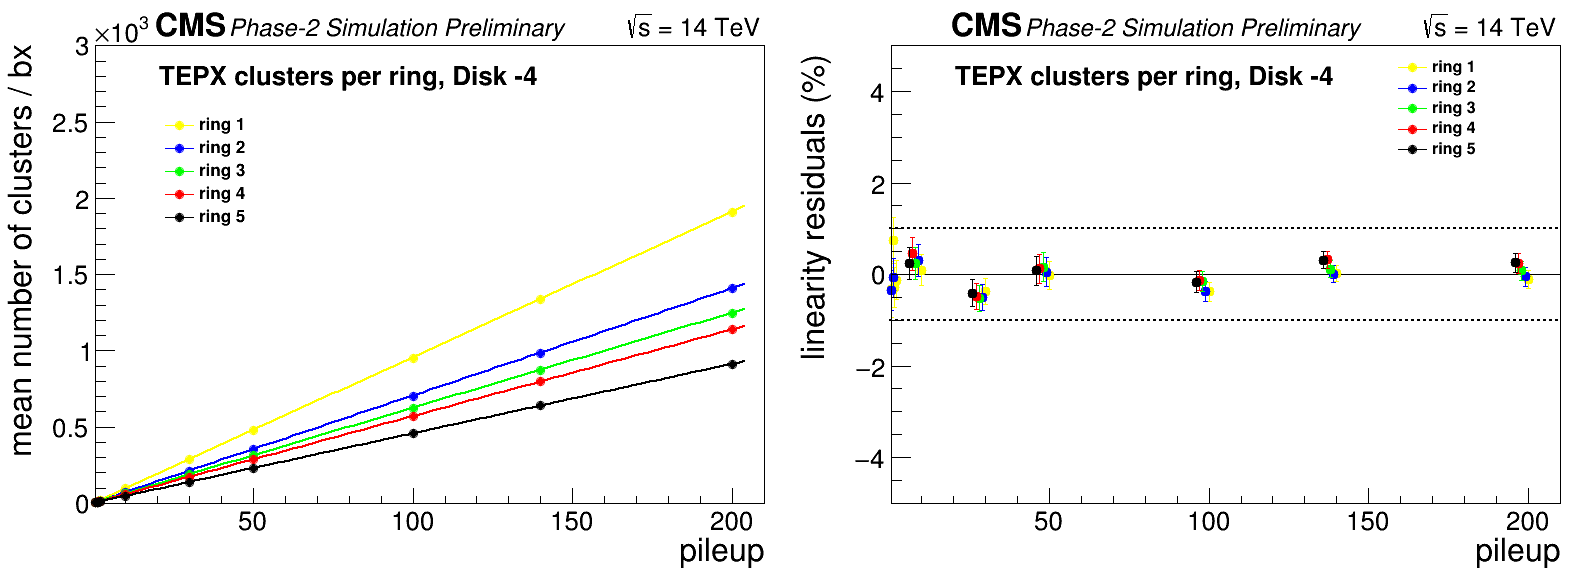
\includegraphics[width=1\columnwidth]{./clustersperringD-4.png}
  \caption{Left: Simulated mean number of clusters for TEPX Disk 4 all rings as a function of pileup. Ring 1 has highest slope and Ring 5 has least slope. Right: Deviation from linearity for clusters for TEPX Disk 4 all rings. Non-linearity is within $1\%$ for all rings over entire pileup range.}
  \label{fig:CMS}
\end{figure}

\begin{figure}[H]
  \centering
  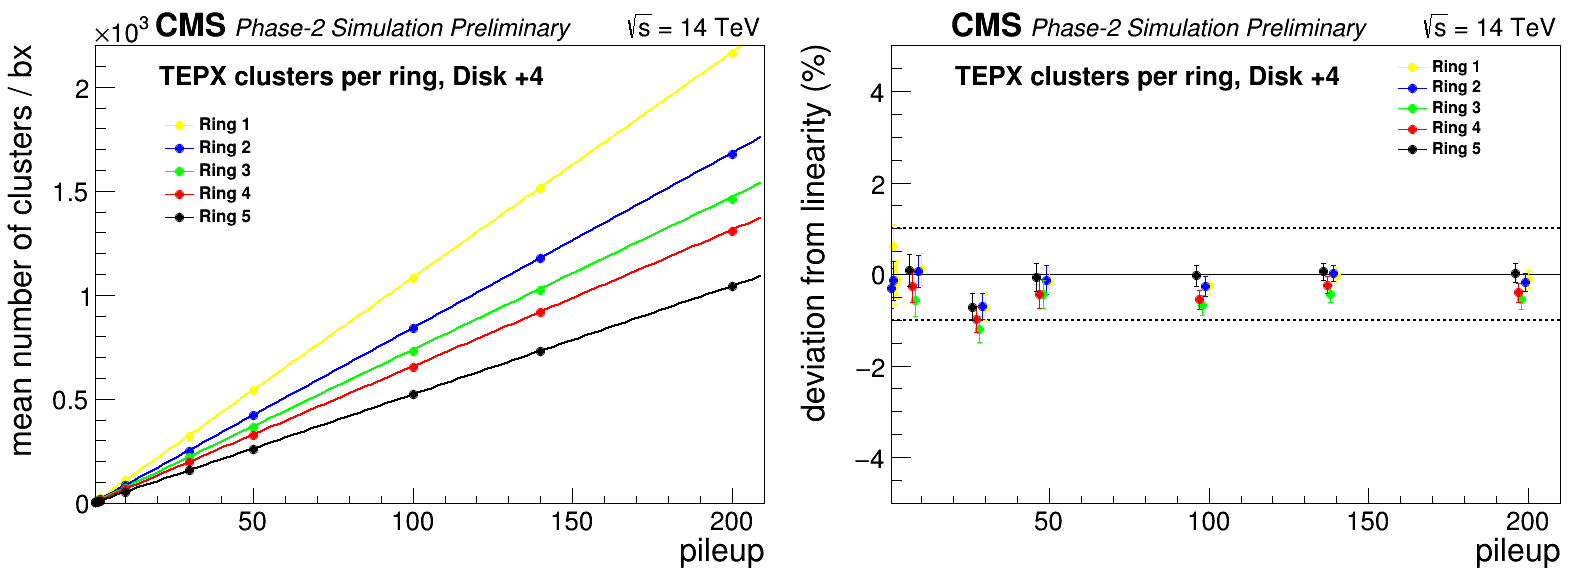
\includegraphics[width=1\columnwidth]{./clustersperringD+4.png}
  \caption{Left: Simulated mean number of clusters for TEPX Disk 4 all rings as a function of pileup. Ring 1 has highest slope and Ring 5 has least slope. Right: Deviation from linearity for clusters for TEPX Disk 4 all rings. Non-linearity is within $1\%$ for all rings over entire pileup range.}
  \label{fig:CMS}
\end{figure}



\begin{figure}[H]
  \centering
  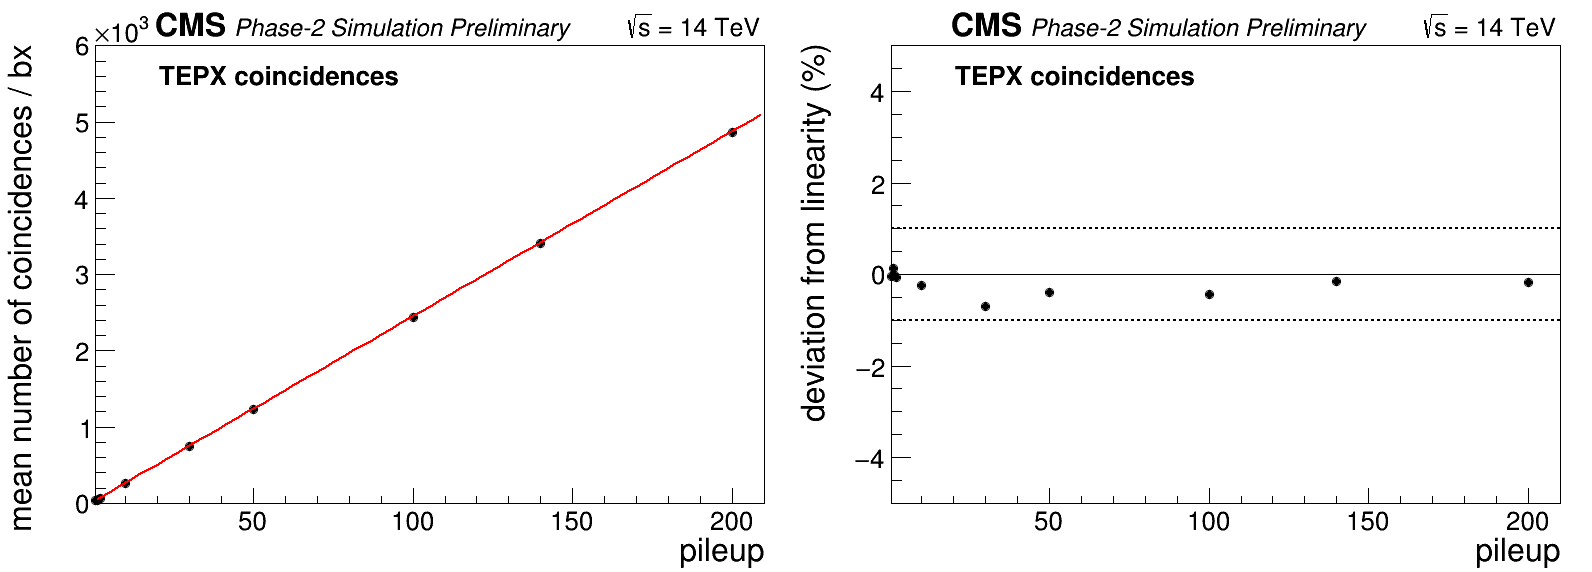
\includegraphics[width=1 \columnwidth]{./totalcoincidences.png}
  \caption{Left: Simulated mean number of coincidences in $\phi$ and r for all entire TEPX detector as a function of pileup. A line is fitted between pileup values of 0 and 2, and then extrapolated up to a pileup of 200. Right: Deviation from linearity for coincidence in $\phi$ and r for entire TEPX detector. The non-linearity is calculated as the relative difference between the data points and the values of the fit function at the respective pileup value. Non-linearity is within 1 \% for entire pileup range. Pileup 200 corresponds to High Luminosity (HL)-LHC environment.}
  \label{fig:CMS}
\end{figure}


\begin{figure}[H]
  \centering
  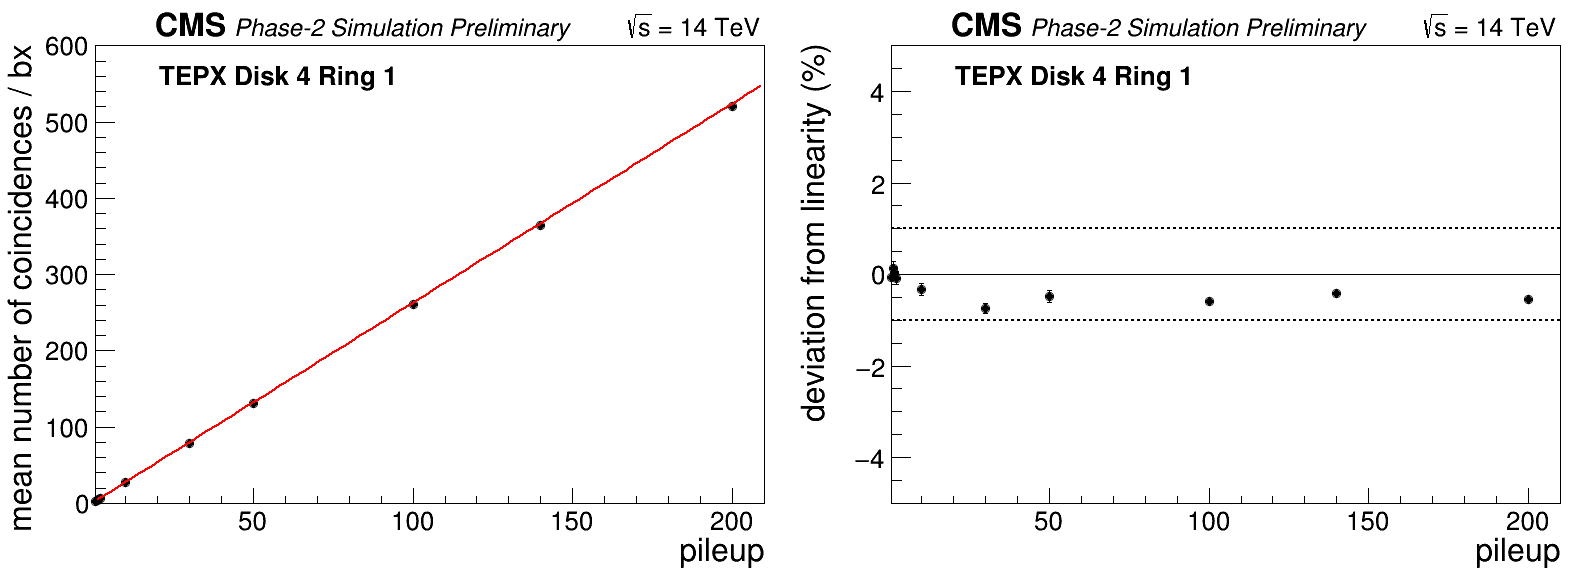
\includegraphics[width=1\columnwidth]{./totalcoincidencesD4R1.png}
  \caption{Left: Simulated mean number of coincidences in $\phi$ and r for TEPX Disk 4 Ring 1 as a function of pileup. Right: Deviation from linearity for coincidences in $\phi$ and r for TEPX Disk 4 Ring 1. The non-linearity is calculated as the relative difference between the data points and the values of the fit function at the respective pileup value.}
  \label{fig:CMS}
\end{figure}


\begin{figure}[H]
  \centering
  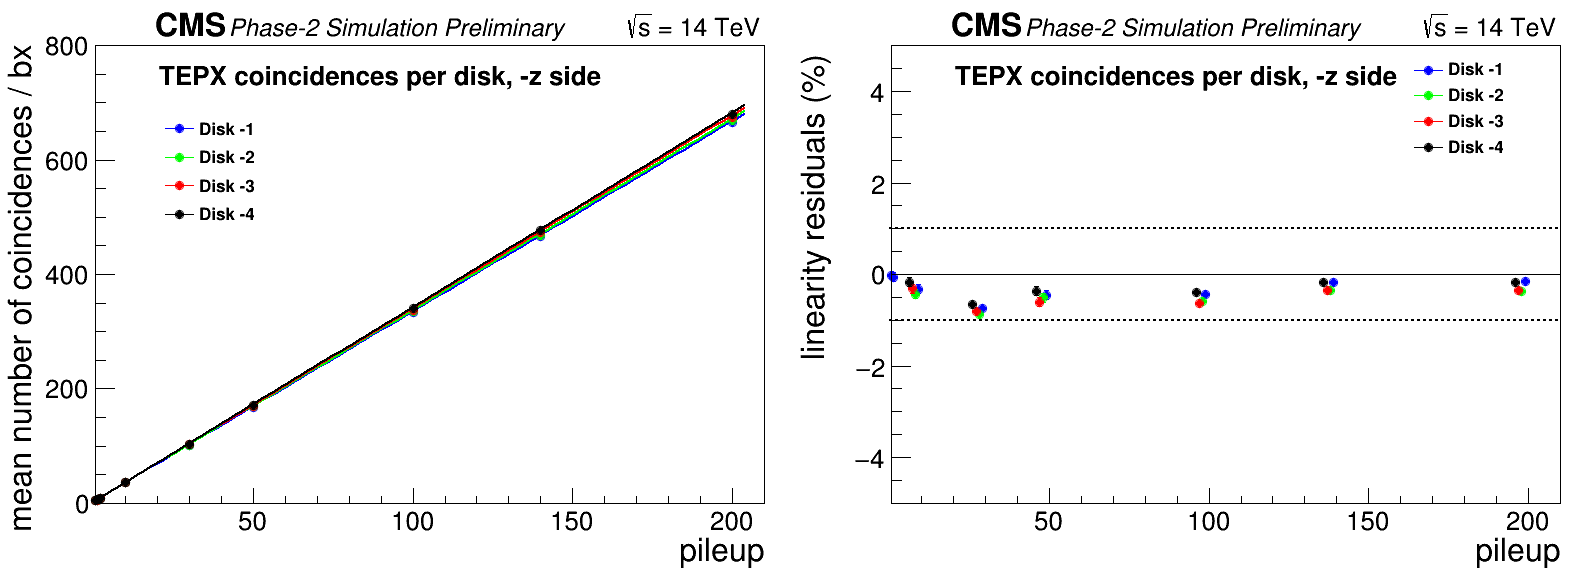
\includegraphics[width=1\columnwidth]{.//coincidencesperdisk-z.png}
  \caption{Left: Simulated mean number of coincidences in $\phi$ and r for -z side TEPX disks as a function of pileup. Right: Deviation from linearity for coincidences in $\phi$ and r for -z side TEPX disks.}
  \label{fig:CMS}
\end{figure}


\begin{figure}[H]
  \centering
  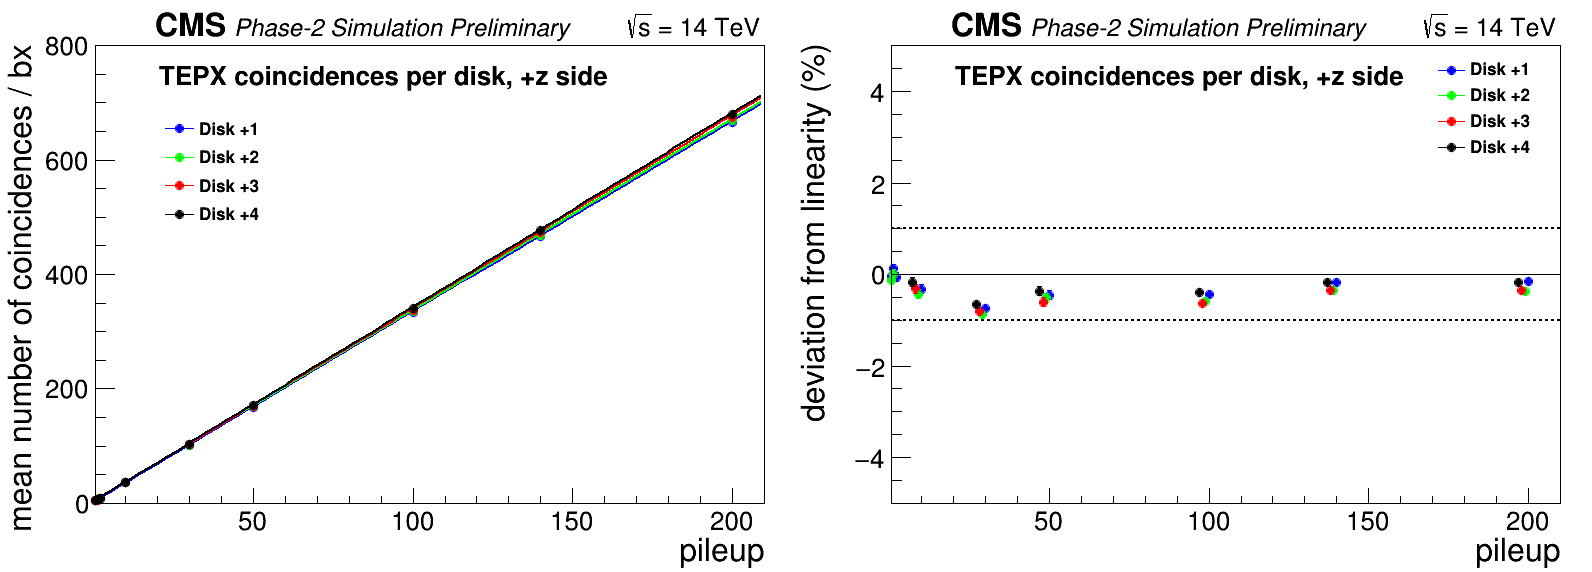
\includegraphics[width=1\columnwidth]{./coincidencesperdisk+z.png}
  \caption{Left: Simulated mean number of coincidences in $\phi$ and r for +z side TEPX disks as a function of pileup. Right: Deviation from linearity for coincidences in $\phi$ and r for +z side TEPX disks.}
  \label{fig:CMS}
\end{figure}







\begin{figure}[H]
  \centering
  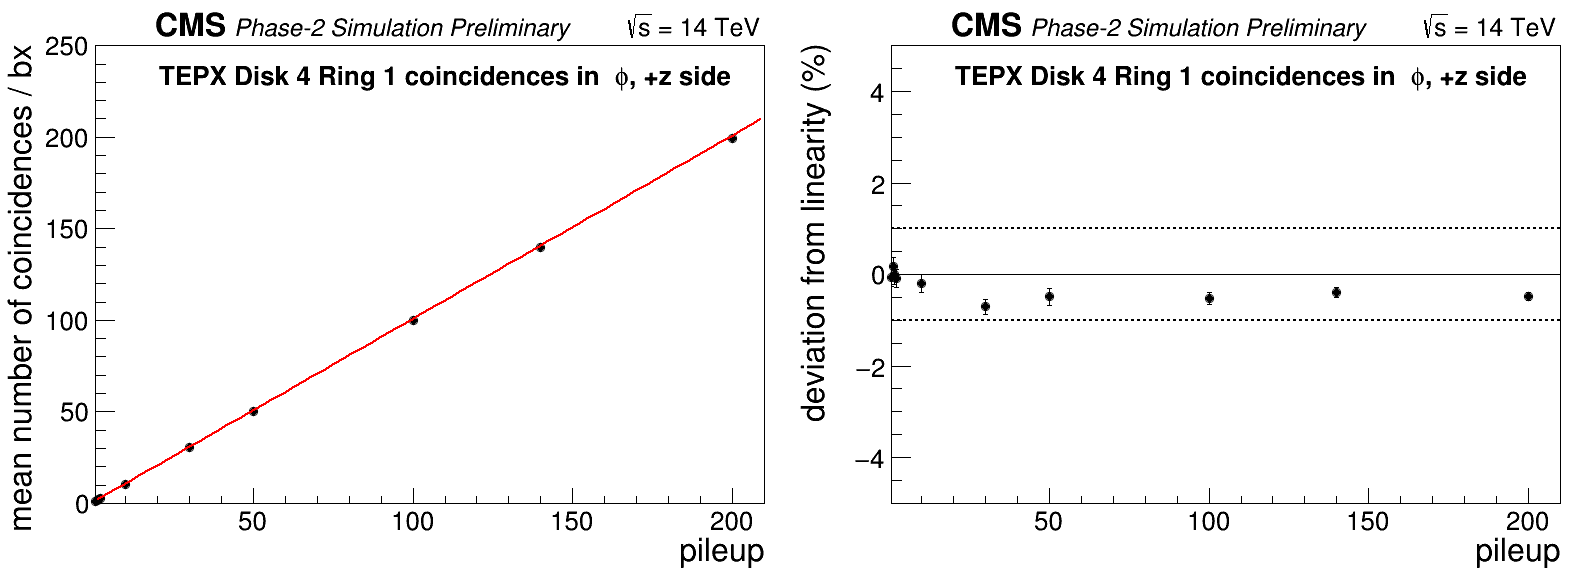
\includegraphics[width=1\columnwidth]{./coincidencesinphiD4R1z+.png}
  \caption{Left: Simulated mean number of coincidences in $\phi$ for TEPX +z side Disk 4 Ring 1 as a function of pileup. Right: Deviation from linearity for coincidences in $\phi$ for TEPX +z side Disk 4 Ring 1. The non-linearity is calculated as the relative difference between the data points and the values of the fit function at the respective pileup value.}
  \label{fig:CMS}
\end{figure}



\begin{figure}[H]
  \centering
  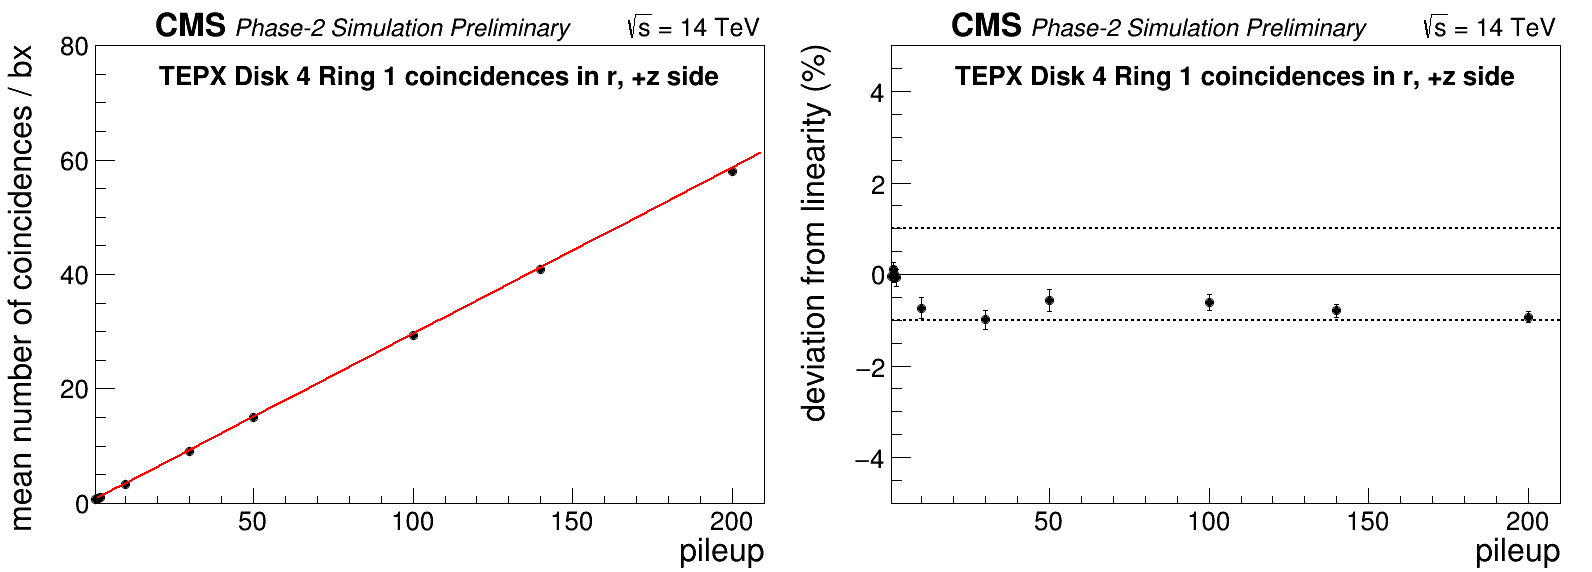
\includegraphics[width=1\columnwidth]{./coincidencesinrD4R1z+.png}
  \caption{Left: Simulated mean number of coincidences in r for TEPX +z side Disk 4 Ring 1 as a function of pileup. Right: Deviation from linearity for coincidences in r for TEPX +z side Disk 4 Ring 1. The non-linearity is calculated as the relative difference between the data points and the values of the fit function at the respective pileup value.}
  \label{fig:CMS}
\end{figure}


\begin{figure}[H]
  \centering
  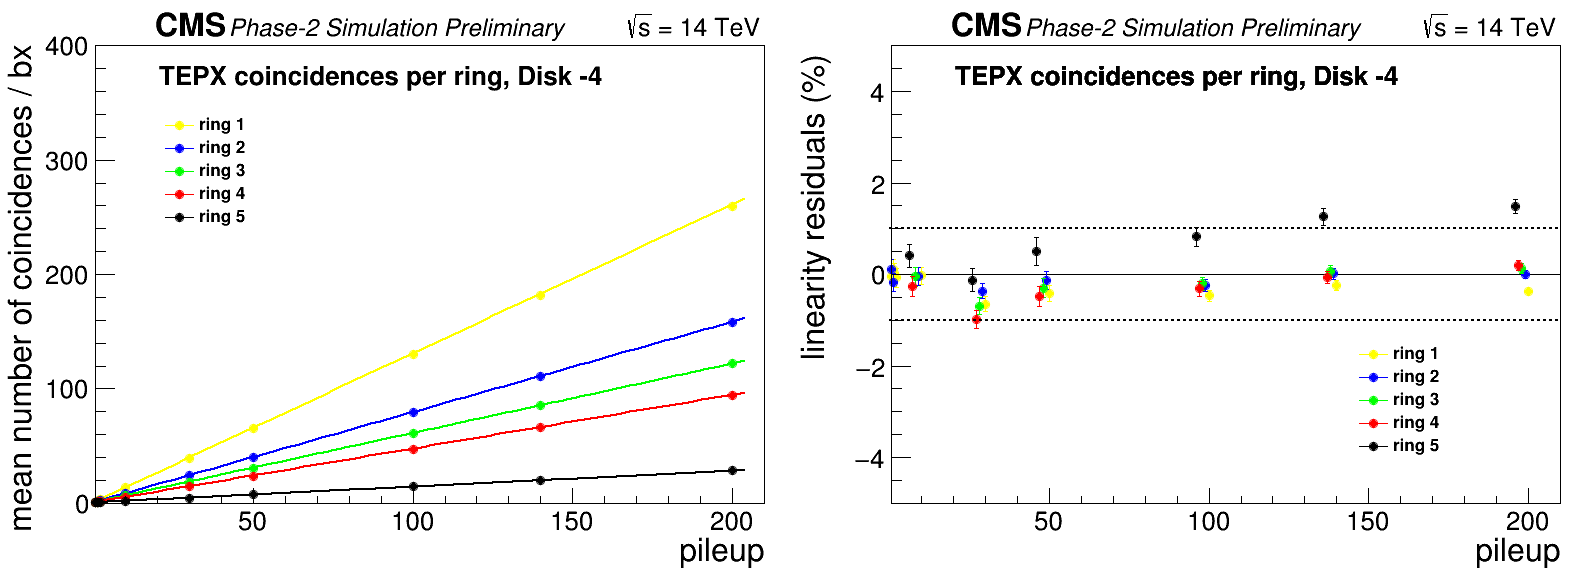
\includegraphics[width=1\columnwidth]{./coincidencesperringD-4.png}
  \caption{Left: Simulated mean number of coincidences in $\phi$ and r for -z side TEPX Disk 4 per ring as a function of pileup. Ring 1 has highest slope and Ring 5 has least slope. Right: Deviation from linearity for coincidences in $\phi$ and r for -z side TEPX Disk 4 per ring. Non-linearity is within 1\% for all rings over entire pileup range.}
  \label{fig:CMS}
\end{figure}


\begin{figure}[H]
  \centering
  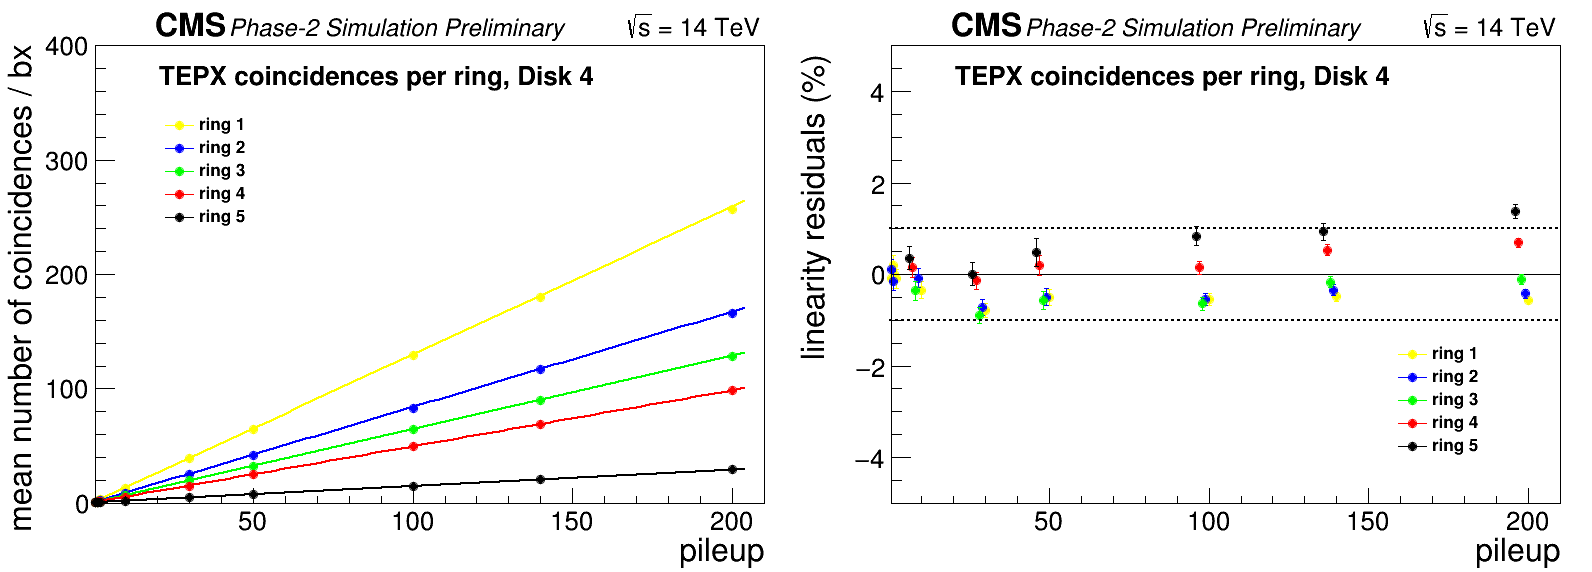
\includegraphics[width=1\columnwidth]{./coincidencesperringD+4.png}
  \caption{Left: Simulated mean number of coincidences in $\phi$ and r for +z side TEPX Disk 4 per ring as a function of pileup. Ring 1 has highest slope and Ring 5 has least slope. Right: Deviation from linearity for coincidences in $\phi$ and r for +z side TEPX Disk 4 per ring. Non-linearity is within 1\% for all rings over entire pileup range.}
  \label{fig:CMS}
\end{figure}






\begin{figure}[H]
  \centering
  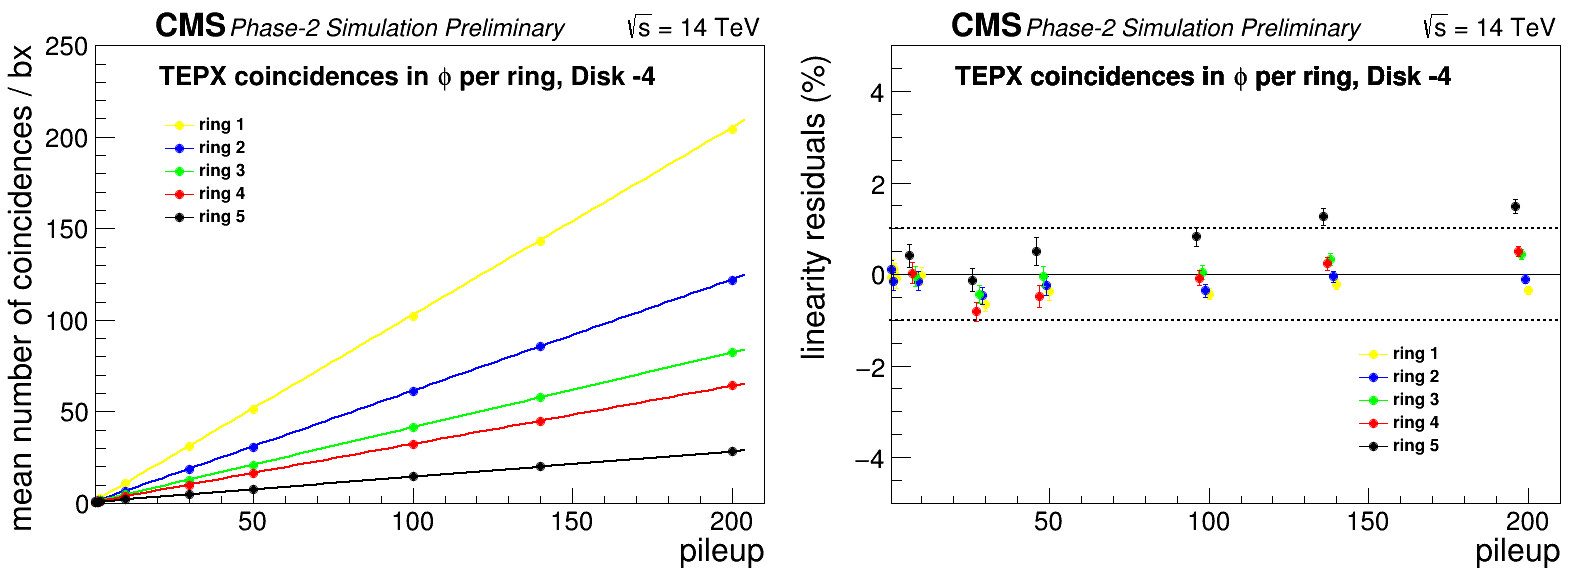
\includegraphics[width=1\columnwidth]{./coincidencesinphiperringD-4.png}
  \caption{Left: Simulated mean number of coincidences in $\phi$ for -z side TEPX Disk 4 per ring as a function of pileup. Ring 1 has highest slope and Ring 5 has least slope. Right: Deviation from linearity for coincidences in $\phi$ for -z side TEPX Disk 4 per ring. Non-linearity is within 1\% for all rings over entire pileup range.}
  \label{fig:CMS}
\end{figure}

\begin{figure}[H]
  \centering
  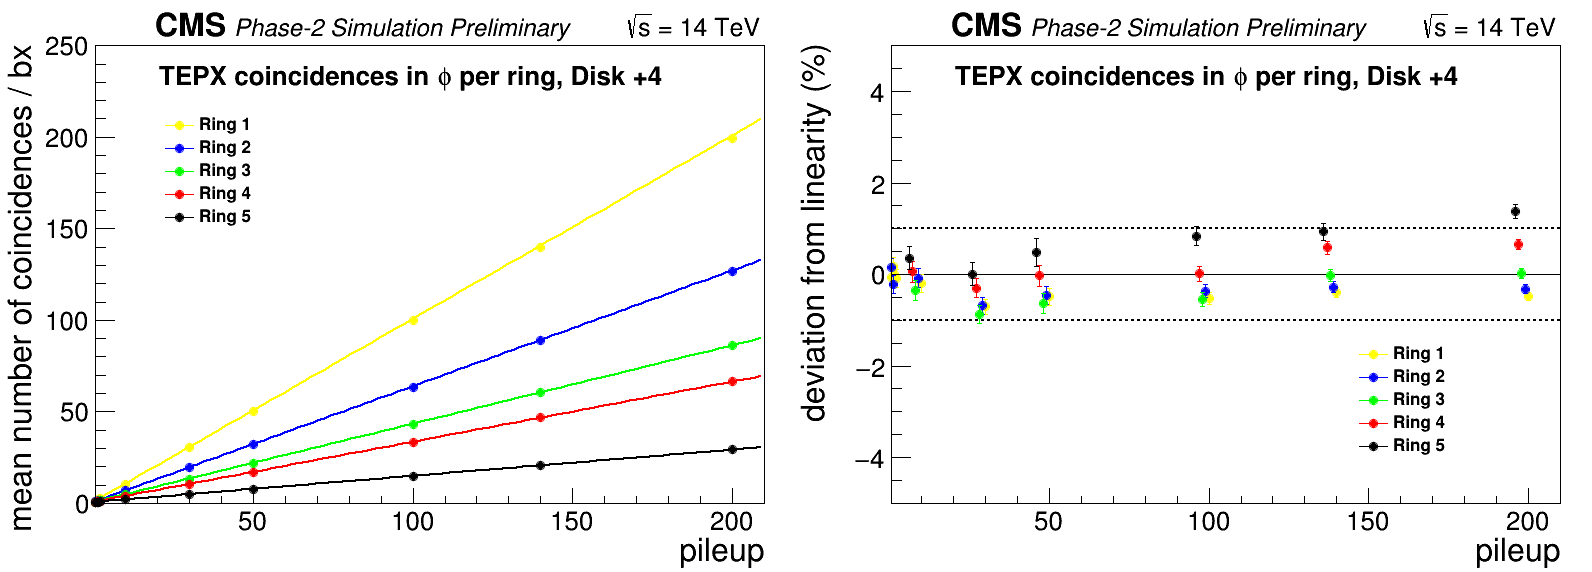
\includegraphics[width=1\columnwidth]{./coincidencesinphiperringD+4.png}
  \caption{Left: Simulated mean number of coincidences in $\phi$ for +z side TEPX Disk 4 per ring as a function of pileup. Ring 1 has highest slope and Ring 5 has least slope. Right: Deviation from linearity for coincidences in $\phi$ for +z side TEPX Disk 4 per ring. Non-linearity is within 1\% for all rings over entire pileup range.}
  \label{fig:CMS}
\end{figure}


\begin{figure}[H]
  \centering
  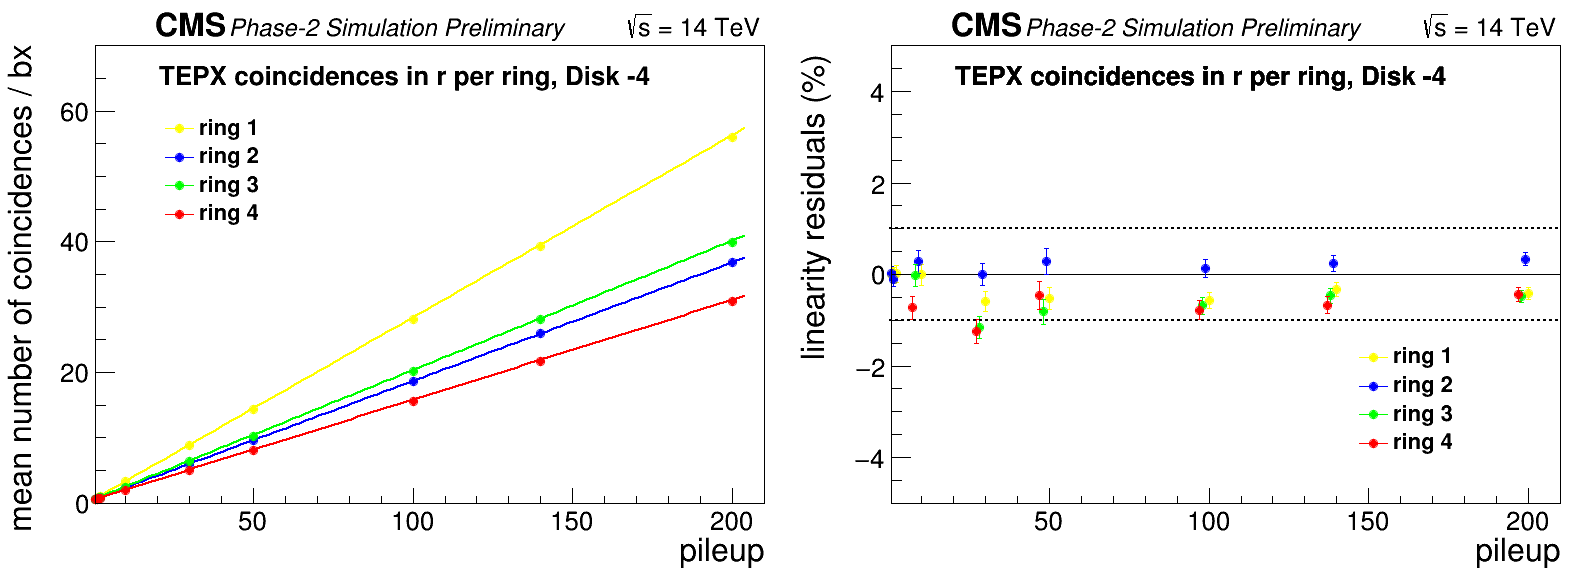
\includegraphics[width=1\columnwidth]{./coincidencesinrperringD-4.png}
  \caption{Left: Simulated mean number of coincidences in r for -z side TEPX Disk 4 per ring as a function of pileup. Ring 1 has highest slope and Ring 5 has least slope. Right: Deviation from linearity for coincidences in r for -z side TEPX Disk 4 per ring. Non-linearity is within $1\%$ for all rings over entire pileup range.}
  \label{fig:CMS}
\end{figure}


\begin{figure}[H]
  \centering
  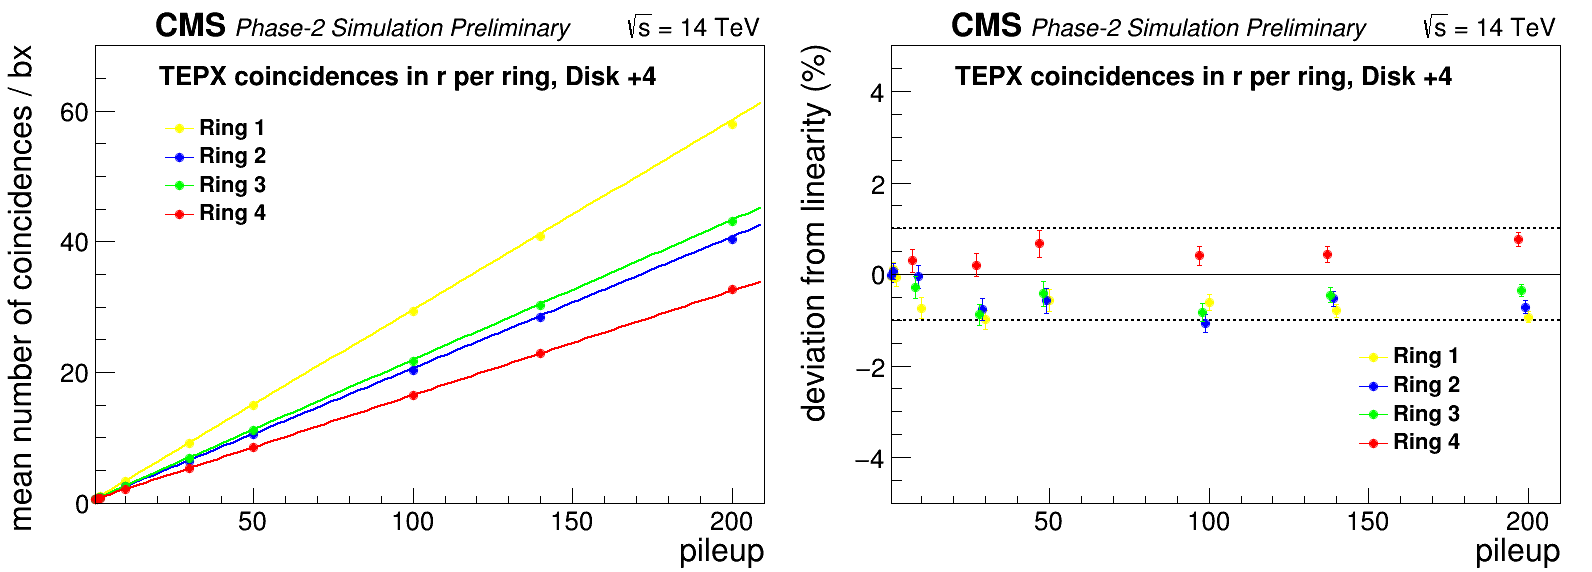
\includegraphics[width=1\columnwidth]{./coincidencesinrperringD+4.png}
  \caption{Left: Simulated mean number of coincidences in r for +z side TEPX Disk 4 per ring as a function of pileup. Ring 1 has highest slope and Ring 5 has least slope. Right: Deviation from linearity for coincidences in r for +z side TEPX Disk 4 per ring. Non-linearity is within $1\%$ for all rings over entire pileup range.}
  \label{fig:CMS}
\end{figure}







VdM (PU 0.5) $\:\:$  Trigger frequency (kHz) $\:\:$ 1 bx, 30 s $\:\:$ 100 bx, 30 s \\
TEPX D4R1 2x Coincidences in $\phi$  $\:\:$  800        $\:\:$   1.7         $\:\:$       0.17   \\
TEPX 2x Coincidences in $\phi$   $\:\:$     500        $\:\:$   0.485       $\:\:$       0.0485   \\




Physics (PU 200)  $\:\:$ Trigger frequency (kHz)   $\:\:$   1 bx, 4 LN (1.46 s)   $\:\:$     2500 bx, 1 LS (23 s)  \\
                                                      $\:\:$           ``Online''          $\:\:$           ``Offline''      \\
TEPX D4R1 2x Coincidences in $\phi$  $\:\:$   800                $\:\:$   0.386           $\:\:$            0.00193         \\
TEPX 2x Coincidences in $\phi$       $\:\:$   75           $\:\:$         0.284           $\:\:$            0.00142         \\

